\input templates/header
\title[ASD - Backtracking]{\textbf{Algoritmi e Strutture Dati}\\[24pt]Backtracking}

\usepackage[mode=buildnew]{standalone}
\usepackage{xcolor}
\usepackage{colortbl}
\usepackage{epigraph}
\usepackage{tikz}
\usepackage{xmpmulti}
\usepackage{listings}

\newcommand{\R}[1]{\textcolor{red}{#1}}
\newcommand{\B}[1]{\textcolor{blue}{#1}}

\renewcommand{\arraystretch}{1.4}
\graphicspath{{figs/16/}}

\renewcommand{\enumerazione}{\fontproc{enumeration}}
\newcommand{\isAdmissible}{\fontproc{accept}}
\newcommand{\isImpossible}{\fontproc{reject}}

\begin{document}


%-------------------------------------------------------------------------
\FrameTitle{}

%-------------------------------------------------------------------------
\FrameContent



%%%%%%%%%%%%%%%%%%%%%%%%%%%%%%%%%%%%%%%%%%%%%%%%%%%%%%%%%%%%%%%%%%%%%%%%%%
\section{Introduzione}

%-------------------------------------------------------------------------
\begin{frame}{Soluzioni ammissibili e soluzioni ottime}

\vspace{-9pt}
\begin{myboxtitle}[Soluzione ammissibile]
Dato un problema, una \alert{soluzione ammissibile} è una soluzione che \alert{soddisfa un insieme di criteri}
\BIL
\item \alert{Zaino}: sottoinsieme di oggetti di peso inferiore alla capacità
\item \alert{Sottosequenza} comune: una stringa che è sottosequenza di entrambe le stringhe in input
\EIL
\end{myboxtitle}

 
\begin{myboxtitle}[Valutare le soluzioni ammissibili]
Nei problemi di ottimizzazione, viene definita una \alert{funzione di\\ costo/guadagno} definita sull'insieme delle soluzioni ammissibili
\BIL
\item \alert{Zaino}: somma dei guadagni degli oggetti selezionati
\item \alert{Sottosequenza comune massimale}: lunghezza della stringa
\EIL
\end{myboxtitle}

\end{frame}

%---------------------------------------------------------------------------
\begin{frame}{Brute-force}

\vspace{-9pt}
\begin{myboxtitle}[Esplorazione]
In alcuni problemi è richiesto o necessario \alert{esplorare l'intero spazio delle soluzioni ammissibili}.
\end{myboxtitle}

\vspace{-9pt}
\begin{overprint}
%----------------------------------
\onslide<1|handout:1>
\begin{columns}[T]
\column{0.62\textwidth}
\begin{myboxtitle}[Enumerazione]
Elencare \alert{tutte} le soluzioni ammissibili

\medskip
\alert{Esempio}: Elencare tutte le permutazioni di un insieme

\medskip
\alert{Soluzione}: Algoritmi di enumerazione

\end{myboxtitle}
\column{0.35\textwidth}
\bigskip
\begin{align*}
    [ 1, 2, 3 ] \\
    [ 1, 3, 2 ] \\
    [ 2, 1, 3 ] \\
    [ 2, 3, 1 ] \\
    [ 3, 2, 1 ] \\
    [ 3, 1, 2 ] 
\end{align*}
\end{columns}
%----------------------------------
\onslide<2|handout:2>
\begin{columns}[T]
\column{0.62\textwidth}
\begin{myboxtitle}[Ricerca]
Trovare \alert{una} soluzione ammissibile in uno spazio delle soluzioni molto grande

\medskip
\alert{Esempio}: Trovare una sequenza di mosse per il gioco del 15

\medskip
\alert{Soluzione}: Algoritmi di enumerazione, fermandosi alla prima soluzione trovata
\end{myboxtitle}
\column{0.33\textwidth}
\begin{center}
\IG{0.9}{15.png}
\end{center}
\end{columns}

\medskip
\tiny
\url{https://it.wikipedia.org/wiki/Gioco_del_quindici\#/media/File:15-puzzle.svg}
%----------------------------------
\onslide<3|handout:3>
\begin{columns}[T]
\column{0.62\textwidth}
\begin{myboxtitle}[Conteggio]
Contare tutte le soluzioni ammissibili

\medskip
\alert{Esempio}: contare il numero di modi in cui è possibile esprimere un
valore $n$ come somma di $k$ numeri primi.

\medskip
\alert{Soluzione}: Se non è possibile contare in modo analitico, bisogna enumerare tutte le soluzioni ammissibili e contarle.
\end{myboxtitle}
\column{0.35\textwidth}

\bigskip
\bigskip
\alert{Input}: $n=23, k=2$\\
\alert{Output}: $2$

\begin{align*}
  23 &= 3+7+13\\
     &= 5+7+11
\end{align*}
\end{columns}
%----------------------------------
\onslide<4|handout:4>
\begin{columns}[T]
\column{0.72\textwidth}
\begin{myboxtitle}[Ottimizzazione]
Trovare una delle soluzioni ammissibili migliori (\alert{ottimizzazione}) rispetto ad un certo criterio di valutazione

\medskip
\alert{Esempio}: trovare il cammino di peso massimo da $s$ a $d$
in un grafo pesato

\medskip
\alert{Soluzione}: Enumerare tutti i cammini da $s$ a $d$, restituire quello
di peso massimo
\end{myboxtitle}
\column{0.25\textwidth}
\scalebox{0.67}{
\includestandalone{figs/16/maxpath}
}
\end{columns}
%----------------------------------

\end{overprint}

\end{frame}

%  Esempio: contare il numero di sottoinsiemi di $k$ elementi presi da un
% insieme di $n$ elementi
% \[
%   \frac{n!}{k!\,(n-k)!}
% \]

%---------------------------------------------------------------------------
\begin{frame}{Costruire tutte le soluzioni è costoso}
\BIL
\item Lo spazio delle possibili soluzioni può avere dimensione superpolinomiale
\item A volte è l'unica strada possibile
\item La potenza dei computer moderni rende "affrontabili" problemi di dimensioni medio-piccole
\BI
\item $10!	= 3.63 \cdot 10^6$	(permutazione di 10 elementi)
\item $2^{20} = 1.05 \cdot 10^6$ (sottoinsieme di 20 elementi)
\EI
\item A nostro vantaggio, a volte lo spazio delle soluzioni non deve essere analizzato interamente
\EIL
\end{frame}

%-------------------------------------------------------------------------
\begin{frame}{Backtracking}

\vspace{-9pt}
\begin{myboxtitle}[Filosofia]
\smallskip
"\emph{Prova a fare qualcosa; se non va  bene, disfalo e prova qualcos'altro}"

\smallskip
"\emph{Ritenta, e sarai più fortunato}"
\end{myboxtitle}

\vspace{-14pt}
\begin{columns}
\column{0.50\textwidth}
\begin{myboxtitle}[Ricorsione]
Un metodo \alert{sistematico} per esplorare uno spazio di ricerca, utilizzando la ricorsione per memorizzare le scelte fatte finora\\[-4pt]
\end{myboxtitle}
\column{0.46\textwidth}
\begin{myboxtitle}[Iterazione]
Utilizza un approccio greedy, eventualmente tornando sui propri passi
\BI
\item \alert{Inviluppo convesso}
\item String matching
\EI
\end{myboxtitle}
\end{columns}

\BB{
Una tecnica algoritmica che, come altre, deve essere personalizzata per ogni applicazione individuale
}

\end{frame}

%%%%%%%%%%%%%%%%%%%%%%%%%%%%%%%%%%%%%%%%%%%%%%%%%%%%%%%%%%%%%%%%%%%%%%%%%%%%
\section{Enumerazione}
%%%%%%%%%%%%%%%%%%%%%%%%%%%%%%%%%%%%%%%%%%%%%%%%%%%%%%%%%%%%%%%%%%%%%%%%%%%%

%---------------------------------------------------------------------------
\begin{frame}{Organizzazione generale}
    
\begin{myboxtitle}[Organizzazione generale]
\BI
\item Una soluzione viene rappresentata come un \alert{vettore di scelte $S[1 \ldots n]$} 
\item  Il contenuto degli elementi $S[i]$ è preso da un \alert{insieme di scelte $C$} dipendente dal problema 
\EI
\end{myboxtitle}

\begin{myboxtitle}[Esempi]
\BI
\item $C$ elementi di un insieme, possibili soluzioni \alert{sottoinsiemi} di $C$
\item $C$ elementi di un insieme, possibili soluzioni \alert{permutazioni} di $C$
\item $C$ mosse di gioco, possibili soluzioni \alert{sequenze di mosse}
\item $C$ archi di un grafo, possibili soluzioni \alert{percorsi sul grafo}
\EI
\end{myboxtitle}

\end{frame}


%---------------------------------------------------------------------------
\begin{frame}{Enumerazione -- Schema parziale}

\vspace{-9pt}
\begin{Procedure}
\caption[A]{\textcolor{violet}{\enumerazione}($\langle \mathit{dati\ problema} \rangle$, $\Item[\,]\ S$, \INTEGER\ $i$, $\langle \mathit{dati\ parziali} \rangle)$}
\Comment{Verifica se $S[1 \ldots i-1]$ contiene una soluzione ammissibile}
\eIf{$\textcolor{violet}{\isAdmissible}(\langle \mathit{dati\ problema} \rangle, S, i, \langle \mathit{dati\ parziali} \rangle)$}
{
  \Comment{"Processa" la soluzione (stampa, conta, etc.)}
  $\textcolor{violet}{\processSolution}(\langle \mathit{dati\ problema} \rangle, S, i, \langle \mathit{dati\ parziali} \rangle)$\;
}
{
  \Comment{Calcola l'insieme delle scelte in funzione di $S[1 \mldots i-1]$}
  $\Set\ C = \textcolor{violet}{\getChoices}(\langle \mathit{dati\ problema} \rangle, S, i, \langle \mathit{dati\ parziali} \rangle)$\;
  \Comment{Itera sull'insieme delle scelte}
  \ForEach{$c \in C$}
  {
    $S[i] = c$\;
    \Comment{Chiamata ricorsiva}
    $\textcolor{violet}{\enumerazione}(\langle \mathit{dati\ problema} \rangle, S, i+1, \langle \mathit{dati\ parziali} \rangle)$
  }
}
\end{Procedure}

\end{frame}

%---------------------------------------------------------------------------
\begin{frame}{Soluzioni parziali}

\BIL
\item Il parametro $i$ rappresenta l'indice della prossima decisione da prendere
\item La soluzione parziale $S[1 \ldots i-1]$ contiene le decisioni prese finora
\item \alert{Caso base}: 
  \BI
  \item Se $S[1 \ldots i-1]$ è una soluzione ammissibile, questa   viene processata
  \item Assumendo che le soluzioni ammissibili non possano essere estese, la ricorsione termina 
  \EI
\item \alert{Passo ricorsivo}  
  \BI
  \item Altrimenti, calcoliamo l'insieme $C$ delle scelte possibili 
  \item Per ogni elemento $c \in C$:
    \BI
    \item Scriviamo $c$ sulla scelta $S[i]$
    \item Chiamiamo ricorsivamente la funzione con indice $i+1$
    \EI
  \EI
\EIL

\end{frame}

\begin{frame}{Albero delle decisioni}

\BI
\item \alert{Albero di decisione} $\equiv$ Spazio di ricerca
\item \alert{Radice} $\equiv$ Soluzione parziale vuota
\item \alert{Nodi interni dell'albero di decisione} $\equiv$ Soluzioni parziali  
\item \alert{Foglie in un albero di decisione} $\equiv$ Soluzioni ammissibili 
\EI

\medskip
\begin{overprint}
\onslide<1|handout:0>\centerline{\includestandalone{figs/16/albero01}}
\onslide<2|handout:0>\centerline{\includestandalone{figs/16/albero02}}
\onslide<3|handout:0>\centerline{\includestandalone{figs/16/albero03}}
\onslide<4|handout:0>\centerline{\includestandalone{figs/16/albero04}}
\onslide<5|handout:0>\centerline{\includestandalone{figs/16/albero05}}
\onslide<6|handout:0>\centerline{\includestandalone{figs/16/albero06}}
\onslide<7|handout:0>\centerline{\includestandalone{figs/16/albero07}}
\onslide<8|handout:0>\centerline{\includestandalone{figs/16/albero08}}
\onslide<9|handout:0>\centerline{\includestandalone{figs/16/albero09}}
\onslide<10|handout:1>\centerline{\includestandalone{figs/16/albero10}}
\end{overprint}

\end{frame}


\subsection{Sottoinsiemi e permutazioni}

%---------------------------------------------------------------------------
\begin{frame}{Sottoinsiemi}

\vspace{-9pt}
\BB{Elencare tutti i sottoinsiemi dell'insieme $\{ 1, \ldots, n \}$}

\vspace{-12pt}
\begin{columns}[T]
\column{0.48\textwidth}    
\begin{Procedure}
\caption[A]{\fontproc{subsetsRec}(\INTEGER $n$, $\INTEGER[\,]\ S$, \INTEGER $i$)}
\Comment{$S$ ammissibile dopo $n$ scelte}
\eIf{$i > n$}{
  $\processSolution(S,n)$\;
}{
  \Comment{Non presente / presente}
  $\Set\ C = \{ 0, 1 \}$\;
  \ForEach{$c \in C$}{
    $S[i] = c$\;
  	$\fontproc{subsetsRec}(n, S, i+1)$\;
  }
}
\end{Procedure}
\column{0.48\textwidth}    
\begin{Procedure}
\caption[A]{\enumerasottoinsiemi(\INTEGER $n$)}
\Comment{Vettore delle scelte}
$\INTEGER[\,]\ S = \NEW\ \INTEGER[1 \ldots n]$\;
$\fontproc{subsetsRec}(n, S,1)$\;
\end{Procedure}

\vspace{-12pt}
\begin{Procedure}
\caption[A]{\processSolution($\INTEGER[\,]\ S$, \INTEGER $n$)}
  \PRINT "\{ "\;
  \For{$i = 1$ \TO\ $n$}{
    \If{$S[i]$}{
      \PRINT $i$, " "\;
    }
  }    
  \PRINTLN "\}"
\end{Procedure}

\end{columns}

\end{frame}

%---------------------------------------------------------------------------
\begin{frame}{Sottoinsiemi -- Note}
	
\BIL
\item Come richiesto dal problema, tutto lo spazio possibile viene esplorato
\item Complessità $\Theta(n \cdot 2^n)$
\item In che ordine vengono stampati gli insiemi?
\EIL

\end{frame}

%---------------------------------------------------------------------------
\begin{frame}{Sottoinsiemi -- Albero delle decisioni}

\begin{center}
\scalebox{1.5}{
\includestandalone{figs/16/albero-sottoinsiemi}
}
\end{center}

\end{frame}






%---------------------------------------------------------------------------
\begin{frame}{Sottoinsiemi -- Versione iterativa}

\vspace{-9pt}
\BB{\EE possibile risolvere questo problema in modo iterativo?}

\pause
\begin{Procedure}
\caption[A]{\enumerasottoinsiemi(\INTEGER $n$)}
\For{$j = 0$ \TO $2^{n}-1$}{
  \PRINT\ "\{ "\;
  \For{$i = 0$ \TO $n-1$}{
    \If(\REMF{Bitwise and}){($j$ \texttt{\&\&} $2^i) \neq 0$}{
      \PRINT\ $i$, " "\;
    }
  }
  \PRINTLN\ "\}"\;
}
\end{Procedure}

\vspace{-9pt}
\BB{
Complessità: $\Theta(n \cdot 2^n)$
}


\end{frame}

%---------------------------------------------------------------------------
\begin{frame}{Permutazioni}

\vspace{-9pt}
\BB{Stampa tutte le permutazioni di un insieme $A$}

\vspace{-12pt}
\begin{columns}[T]
\column{0.55\textwidth}
\begin{Procedure}
\caption[A]{\fontproc{permRec}(\Set $A$, $\Item[\,]\ S$, \INTEGER\ $i$)}
\Comment{Se $A$ è vuoto, $S$ è ammissibile}
\eIf{$A.\setempty()$}{
  \PRINT $S$\;
}{
  \Comment{Copia $A$ per il ciclo \textbf{foreach}}
  \Set\ $C = \fontproc{copy}(A)$\;
  \ForEach{$c \in C$}{
    $S[i] = c$\;
    $A.\setremove(c)$\;
    \fontproc{permRec}$(A, S, i+1)$\;
    $A.\setinsert(c)$\;
  }
}
\end{Procedure}
\column{0.41\textwidth}
\begin{Procedure}
\caption[A]{\permutazioni(\Set $A$)}
\INTEGER $n = \setsize(A)$\;
$\INTEGER[\,]\ S = \NEW\ \INTEGER[1 \ldots n]$\;
$\fontproc{permRec}(A,S,1)$\;
\end{Procedure}
\end{columns}
	
\end{frame}

%---------------------------------------------------------------------------
\begin{frame}{Permutazioni -- Albero delle decisioni}

\begin{center}
\scalebox{1.2}{
\includestandalone{figs/16/albero-permutazioni}
}
\end{center}

\end{frame}


%---------------------------------------------------------------------------
\begin{frame}{Permutazioni -- Complessità}

\vspace{-9pt}
\begin{myboxtitle}[Complessità]
\BIL
\item Costo della stampa: $\Theta(n)$
\item Costo delle copie del vettore lungo un cammino radice-foglia:
$
  \sum_{i=1}^n O(i) = O(n^2)
$
\item Numero di foglie: $n!$
\item Complessità $O(n^2 n!)$
\EIL
\end{myboxtitle}

\end{frame}

%---------------------------------------------------------------------------
\begin{frame}{Permutazioni -- Complessità}

\begin{myboxtitle}[Altre implementazioni]
\BIL
\item L'algoritmo più efficiente per generare le permutazioni è l'Algoritmo di Heap 
  \BI
  \item B.R. Heap. \footnote{Sì, esiste un tizio che si chiama Heap di cognome...} "Permutations by Interchanges". The Computer Journal, 6(3):293-294. (1963) [\href{https://academic.oup.com/comjnl/article/6/3/293/360213}{Link}]
  \EI
\item Per i più coraggiosi, Knuth affronta il problema delle permutazioni nel suo Art of Computer Programming \footnote{Solo 66 pagine!}
  \BI
  \item Knuth, Donald. "Section 7.2.1.2: Generating All Permutations", The Art of Computer Programming, volume 4A.  (2011)
  [\href{http://www-cs-faculty.stanford.edu/~uno/fasc2b.ps.gz}{Link}]
  \EI
\EIL
\end{myboxtitle}

\end{frame}

%---------------------------------------------------------------------------
\begin{frame}{Permutazioni -- Una versione più pulita}

\vspace{-9pt}
\BB{Stampa tutte le permutazioni di un vettore $S$}

\vspace{-12pt}
\begin{columns}[T]
\column{0.50\textwidth}
\begin{Procedure}
\caption[A]{\fontproc{permRec}($\Item[\,]\ S$, \INTEGER\ $i$)}
\Comment{Caso base, un elemento}
\eIf{$i \Eq 1$}{
  \PRINTLN $S$\;
}{
  \For{$j = 1$ \TO\ $i$}{
    $\fontproc{swap}(S, i, j)$\;
    $\fontproc{permRec}(S,i-1)$\;
    $\fontproc{swap}(S, i, j)$\;
  }
}
\end{Procedure}
\column{0.46\textwidth}
\begin{Procedure}
\caption[A]{\permutazioni($\Item[\,]\ S$, \INTEGER $n$)}
$\fontproc{permRec}(S,n)$\;
\end{Procedure}

\vspace{-12pt}
\small
\begin{myboxtitle}[Complessità]
\BI
\item $n!$ permutazioni
\item $\Theta(n)$ per stamparle tutte
\item $2n$ swap per ogni permutazione
\item Costo totale $\Theta(n \cdot n!)$
\EI
\end{myboxtitle}

\end{columns}
	
\end{frame}

%---------------------------------------------------------------------------
\begin{frame}{Enumerazione -- Schema completo}

\vspace{-9pt}
\begin{Procedure}
\caption[A]{\textcolor{violet}{\enumerazione}($\langle \mathit{dati\ problema} \rangle$, $\Item[\,]\ S$, \INTEGER\ $i$, $\langle \mathit{dati\ parziali} \rangle)$}
\uIf{$\textcolor{violet}{\isAdmissible}(\langle \mathit{dati\ problema} \rangle, S, i, \langle \mathit{dati\ parziali} \rangle)$}
{
  \Comment{Processo la soluzione $S$ in quanto ammissibile}
  $\textcolor{violet}{\processSolution}(\langle \mathit{dati\ problema} \rangle, S, i, \langle \mathit{dati\ parziali} \rangle)$\;
}
\alert{
\uElseIf{$\textcolor{violet}{\isImpossible}(\langle \mathit{dati\ problema} \rangle, S, i, \langle \mathit{dati\ parziali} \rangle)$}{
    \Return
  }
}
\Else{
  \Comment{Ricorsione}
  $\Set\ C = \textcolor{violet}{\getChoices}(\langle \mathit{dati\ problema} \rangle, S, i, \langle \mathit{dati\ parziali} \rangle)$\;
  \ForEach{$c \in C$}
  {
    $S[i] = c$\;
    $\textcolor{violet}{\enumerazione}(\langle \mathit{dati\ problema} \rangle, S, i+1, \langle \mathit{dati\ parziali} \rangle)$
  }
}
\end{Procedure}

\end{frame}



%---------------------------------------------------------------------------
\begin{frame}{$k$-Sottoinsiemi -- Tentativo 1}

\vspace{-9pt}
\BB{Elencare tutti i sottoinsiemi di $k$ elementi di un insieme $\{ 1, \ldots, n \}$}

\vspace{-12pt}
\begin{columns}[T]
\column{0.58\textwidth}
\begin{Procedure}
\caption[A]{\fontproc{kssRec}(\INTEGER $n$, \INTEGER $k$, $\INTEGER[\,]\ S$, \INTEGER $i$)}
\alert{$\INTEGER\ \mathit{size} = \fontproc{count}(S,n)$}\;
\uIf{$i > n$ \alert{\AND\ $\mathit{size} \Eq k$}}{
  $\processSolution(S, n)$\;
}
\alert{
\uElseIf{$i > n$ \alert{\AND\ $\mathit{size} \neq k$}}{
  $\Return$\;
}
}
\Else{
  \ForEach{$c \in \{ 0, 1 \}$}{
    $S[i] = c$\;
    $\fontproc{kssRec}(n,k, S, i+1)$\;
  }
}
\end{Procedure}
\column{0.41\textwidth}
\begin{Procedure}
\caption[A]{\fontproc{kSubsets}(\INTEGER $n$, \INTEGER $k$)}
$\INTEGER[\,]\ S = \NEW\ \INTEGER[1 \ldots n$]\;
$\fontproc{kssRec}(n,k, S, 1)$\;
\end{Procedure}


\begin{Procedure}
\caption[A]{\INTEGER \fontproc{count}($\INTEGER[\,]\ S$, \INTEGER $n$)}
$\INTEGER\ \Count = 0$\;
\For{$j = 1$ \TO $n$}{
  $\Count = \Count + S[j]$\;
}
\Return $\Count$\;
\end{Procedure}

\end{columns}
\end{frame}

\newcommand{\Missing}{\mathit{missing}}


%---------------------------------------------------------------------------
\begin{frame}{$k$-Sottoinsiemi -- Tentativo 2}
	
\vspace{-9pt}	
\begin{Procedure}
\caption[A]{\fontproc{kssRec}(\INTEGER $n$, \alert{\INTEGER $\Missing$}, $\INTEGER[\,]\ S$, \INTEGER $i$)}
\uIf{$i > n$ \alert{\AND\ $\Missing \Eq 0$}}{
  $\processSolution(S, n)$\;
}
\uElseIf{$i > n$ \alert{\AND\ $\Missing \neq 0$}}{
  $\Return$\;
}
\Else{
  \ForEach{$c \in \{ 0, 1 \}$}{
    $S[i] = c$\;
    $\fontproc{kssRec}(n, \alert{\Missing-c}, S, i+1)$\;
  }
}
\end{Procedure}

\vspace{-12pt}
\begin{myboxtitle}[Note]
\BI
\item Evitiamo di ricontare tutte le volte i bit $1$
\EI
\end{myboxtitle}

\end{frame}

%---------------------------------------------------------------------------
\begin{frame}{$k$-Sottoinsiemi -- Albero delle decisioni, per $n=4, k=2$}

\vspace{-9pt}
\begin{center}
\scalebox{1.0}{
\includestandalone{figs/16/pruning1}
}
\end{center}

\begin{myboxtitle}[Note]
\BI
\item Questa soluzione suggerisce un ulteriore miglioramento...
\item I nodi rossi sono nodi in cui $\Missing$ diventa uguale a zero per la prima volta nel percorso radice--foglia
\EI
\end{myboxtitle}

\end{frame}

%---------------------------------------------------------------------------
\begin{frame}{$k$-Sottoinsiemi -- Tentativo 3 (Pruning parziale)}

\vspace{-9pt}	
\begin{Procedure}
\caption[A]{\fontproc{kssRec}(\INTEGER $n$, \INTEGER $\Missing$, $\INTEGER[\,]\ S$, \INTEGER $i$)}
\uIf{\alert{\xout{$i > n$ \AND}}\ $\Missing \Eq 0$}{
  $\processSolution(S, \alert{i-1})$\;
}
\uElseIf{\alert{$i > n$ \OR\ $\Missing < 0$}}{
  $\Return$\;
}
\Else{
  \ForEach{$c \in \{ 0, 1 \}$}{
    $S[i] = c$\;
    $\fontproc{kssRec}(n, \alert{\Missing-c}, S, i+1)$\;
  }
}
\end{Procedure}

\vspace{-12pt}
\begin{myboxtitle}[Note]
\BI
\item Se $\Missing=0$, la soluzione è ammissibile
\item Non ha senso continuare oltre
\EI
\end{myboxtitle}

\end{frame}

%---------------------------------------------------------------------------
\begin{frame}{Pruning -- Esempio: $n=4, k=2$}

\BIL
\item “Rami” dell'albero che sicuramente non portano a soluzioni ammissibili possono essere “\alert{potati}”  (\alert{pruned})
\item La valutazione viene fatta nelle soluzioni parziali radici del sottoalbero da potare
\EIL

\centerline{\includestandalone{figs/16/pruning2}}

\end{frame}




%---------------------------------------------------------------------------
\begin{frame}{$k$-Sottoinsiemi -- Tentativo 4 (Pruning totale)}
	
\vspace{-9pt}	
\begin{Procedure}
\caption[A]{\fontproc{kssRec}(\INTEGER $n$, \INTEGER $\Missing$, $\INTEGER[\,]\ S$, \INTEGER $i$)}
\uIf{$\Missing \Eq 0$}{
  $\processSolution(S,i-1)$\;
}
\uElseIf{$i > n$ \OR\ $\Missing < 0$ \alert{\OR\ $n-(i-1) < \Missing$}}{
  $\Return$\;
}
\Else{
  \ForEach{$c \in \{ 0, 1 \}$}{
    $S[i] = c$\;
    $\fontproc{kssRec}(n, \Missing-c, S, i+1)$\;
  }
}
\end{Procedure}

\vspace{-12pt}
\begin{myboxtitle}[Note]
\BI
\item Evitiamo di proseguire in rami che non possono dare origine alla soluzione
\EI
\end{myboxtitle}

\end{frame}

%---------------------------------------------------------------------------
\begin{frame}{$k$-Sottoinsiemi -- Albero delle decisioni, per $n=4, k=2$}

\BIL
\item I nodi interni in azzurro rappresentano i nodi che non possono dare origine a soluzioni
\EIL


\begin{center}
\scalebox{1.0}{
\includestandalone{figs/16/pruning3}
}
\end{center}

\end{frame}

%---------------------------------------------------------------------------
\begin{frame}{$k$-Sottoinsiemi -- Tentativo 5 (Clean-up)}
	
\vspace{-9pt}	
\begin{Procedure}
\caption[A]{\fontproc{kssRec}(\INTEGER $n$, \INTEGER $\Missing$, $\INTEGER[\,]\ S$, \INTEGER $i$)}
\uIf{$\Missing \Eq 0$}{
  $\processSolution(S,i-1)$\;
}
\uElseIf{$i \leq n$ \AND\ $0 < \Missing \leq n-(i-1)$}{
  \ForEach{$c \in \{ 0, 1 \}$}{
    $S[i] = c$\;
    $\fontproc{kssRec}(n, \Missing-c, S, i+1)$\;
  }
}
\end{Procedure}

\end{frame}



%---------------------------------------------------------------------------
\begin{frame}{$k$-Sottoinsiemi -- Vantaggi}

\IG{1.0}{plot.pdf}

\end{frame}

%---------------------------------------------------------------------------
\begin{frame}{$k$-Sottoinsiemi -- Sommario}

\BB{Cosa abbiamo imparato?}
\BIL
\item  “Specializzando” l'algoritmo generico, possiamo ottenere una versione più efficiente
\item  Versione efficiente per 
\BI
	\item valori di $k$ “piccoli” (vicini a $1$)
	\item valori di $k$ “grandi” (vicini a $n$)
\EI
\item Miglioramento solo parziale verso $n/2$
\item Possiamo ottenere la stessa efficienza con un algoritmo iterativo?
\EIL
	
\end{frame}

\subsection{Subset sum}

%-------------------------------------------------------------------------
\begin{frame}{Subset Sum}

\vspace{-9pt}
\begin{myboxtitle}[Somma di sottoinsieme (Subset sum)]
Dati un vettore $A$ contenente $n$ interi positivi ed un intero positivo $k$, \alert{esiste} un sottoinsieme $S \subseteq \{ 1 \ldots n\}$ tale che 
$\displaystyle \sum_{i \in S} a[i] = k$?
\end{myboxtitle}

\bigskip
\begin{center}
\begin{tabular}{|c|c|c|c|c|c|c|c|c|}
\hline
i & 1 & 2 & 3 & 4 & 5 & 6 & 7 & 8 \\\hline
A & 1 & \alert{4} & 3 & \alert{12} & \alert{7} & \textcolor{blue}{2} &  \textcolor{blue}{21} & 55 \\\hline
\end{tabular}
\end{center}

\begin{align*}
  k &= 23\\
  S_1 &= \{ 2,4,5 \} \\
  S_2 &= \{ 6,7 \}
\end{align*}

\end{frame}

%-------------------------------------------------------------------------
\begin{frame}{Subset Sum}

\vspace{-9pt}
\begin{myboxtitle}[Analisi del problema]
\BIL
\item Lo risolviamo qui tramite backtracking in tempo $O(2^n)$
\item Può essere risolto tramite programmazione dinamica in tempo $O(kn)$
  \BI
  \item Questa complessità è pseudo-polinomiale
  \item Ci torneremo sopra
  \EI
\item \alert{Non siamo interessati a tutte le soluzioni, ce ne basta una}
\item \alert{Interrompiamo l'esecuzione alla prima soluzione trovata}
\EIL
\end{myboxtitle}

\end{frame}

%---------------------------------------------------------------------------
\begin{frame}{Enumerazione -- Interruzione alla prima soluzione}

\vspace{-9pt}
\begin{Procedure}
\caption[A]{\textcolor{violet}{\enumerazione}($\langle \mathit{dati\ problema} \rangle$, $\Item[\,]\ S$, \INTEGER\ $i$, $\langle \mathit{dati\ parziali} \rangle)$}
\uIf{$\textcolor{violet}{\isAdmissible}(\langle \mathit{dati\ problema} \rangle, S, i, \langle \mathit{dati\ parziali} \rangle)$}
{
  $\textcolor{violet}{\processSolution}(\langle \mathit{dati\ problema} \rangle, S, i, \langle \mathit{dati\ parziali} \rangle)$\;
  
  \alert{\Return \TRUE}\REMR{Trovata soluzione, restituisco \TRUE}
}
\uElseIf{$\textcolor{violet}{\isImpossible}(\langle \mathit{dati\ problema} \rangle, S, i, \langle \mathit{dati\ parziali} \rangle)$}{
  \alert{\Return \FALSE}\REMR{Impossibile trovare soluzioni, restituisco \FALSE}
}
\Else{
  $\Set\ C = \textcolor{violet}{\getChoices}(\langle \mathit{dati\ problema} \rangle, S, i, \langle \mathit{dati\ parziali} \rangle)$\;
  \ForEach{$c \in C$}
  {
    $S[i] = c$\;
    \If{$\textcolor{violet}{\enumerazione}(\langle \mathit{dati\ problema} \rangle, S, i+1, \langle \mathit{dati\ parziali} \rangle)$}{
      \alert{\Return \TRUE}\REMR{Trovata soluzione, restituisco \TRUE}
    }
  }
  \alert{\Return \FALSE}\REMR{Nessuna soluzione, restituisco \FALSE}
}
\end{Procedure}

\end{frame}

%---------------------------------------------------------------------------
\begin{frame}{Subset sum}
	
\vspace{-9pt}
\begin{Procedure}
\caption[A]{\BOOLEAN\ \fontproc{ssRec}($\INTEGER[\,]\ A$, \INTEGER $n$, \INTEGER $\Missing$, $\INTEGER[\,]\ S$, \INTEGER $i$)}
\uIf{$\Missing \Eq 0$}{
  $\processSolution(S,i-1)$\REMR{Stampa gli indici della soluzione}
  \Return \TRUE\;
}
\uElseIf{$i > n$ \OR\ $\Missing < 0$}{
  \Return $\FALSE$\REMR{Terminati i valori o somma eccessiva}
}
\Else{
  \ForEach{$c \in \{ 0, 1 \}$}{
    $S[i] = c$\;
    \If{$\fontproc{ssRec}(A, n, \Missing-A[i] \cdot c, S, i+1)$}{
      \Return \TRUE\;
    }
  }
  \Return \FALSE
}
\end{Procedure}

\end{frame}

%---------------------------------------------------------------------------
\begin{frame}{Subset sum}

\vspace{-9pt}
\begin{Procedure}
\caption[A]{\fontproc{subsetSum}($\INTEGER[\,]\ A$, \INTEGER $n$, \INTEGER $k$)}
$\INTEGER[\,]\ S = \NEW\ \INTEGER[1 \ldots n$]\;
$\fontproc{ssRec}(A, n,k, S, 1)$\;
\end{Procedure}

\begin{myboxtitle}[Note]
Avendo informazioni sulle somme cumulative, sarebbe possibile potare ulteriormente
\end{myboxtitle}

\end{frame}

\subsection{Giochi}

%-------------------------------------------------------------------------
\begin{frame}{Problema delle otto regine}

\vspace{-9pt}
\begin{myboxtitle}[Problema]
Posizionare $n$ regine in una scacchiera $n \times n$, in modo tale che 
nessuna regina ne "minacci" un'altra. 
\end{myboxtitle}

\TwoColsCustom{0.58}{0.38}{
\BIL
\item Un po' di storia:
\BI
\item Introdotto da Max Bezzel (1848)
\item Gauss trovò 72 delle 92 soluzioni
\EI
\item Partendo da un approccio "stupido", raffiniamo mano a mano la soluzione
\item L'idea è mostrare l'effetto della modellazione sull'efficenza
\EIL
}{
\vspace{-12pt}
\IG{0.95}{8queen.png}
}
\tiny
\url{https://en.wikipedia.org/wiki/Eight_queens_puzzle}
\end{frame}

%-------------------------------------------------------------------------
\begin{frame}{Problema delle otto regine}

\vspace{-9pt}
\BB{Idea: Ci sono $n^2$ caselle dove piazzare una regina}

\medskip
\begin{tabular}{|P{4cm}|P{7.1cm}|}
\hline
$S[1 \ldots n^2]$ array binario	&	$S[i] = \TRUE \Rightarrow \textrm{"regina in $S[i]$"}$ \\\hline
controllo soluzione	& se $i = n^2$ \\\hline
$\getChoices(S, n, i)$	&	$\{ \TRUE, \FALSE \}$ \\\hline
pruning	&	se la nuova regina minaccia una delle regine esistenti, restituisce $\emptyset$ \\\hline
\# soluzioni per $n=8$ 	&		$\alert{2^{64} \approx 1.84 \cdot 10^{19}}$\\\hline 
\end{tabular}

\begin{myboxtitle}[Commenti]
\BI
\item Forse abbiamo un problema di rappresentazione?
\item Matrice binaria molto sparsa
\EI
\end{myboxtitle}

\end{frame}

%-------------------------------------------------------------------------
\begin{frame}{Problema delle otto regine}

\vspace{-9pt}
\BB{Idea: Dobbiamo piazzare $n$ regine, ci sono $n^2$ caselle}

\medskip
\begin{tabular}{|P{4cm}|P{7.1cm}|}
\hline
$S[1 \ldots n]$ coordinate in $\{ 1 \ldots n^2 \}$	&	$S[i]$ coordinata della regina $i$ \\\hline
controllo soluzione	& se $i = n$ \\\hline
$\getChoices(S, n, i)$	&	$\{ 1 \ldots n^2 \}$ \\\hline
pruning	&	restituisce il sottoinsieme di mosse legali \\\hline
\# soluzioni per $n=8$ 	&		$\alert{(n^2)^n = 64^{8} = 2^{48}  \approx 2.81 \cdot 10^{14}}$\\\hline 
\end{tabular}

\begin{myboxtitle}[Commenti]
\BI
\item C'è un miglioramento, ma lo spazio è ancora grande \ldots
\item Problema: come si distingue una soluzione "1-7-\ldots" da "7-1-\ldots" ?
\EI
\end{myboxtitle}

\end{frame}

%-------------------------------------------------------------------------
\begin{frame}{Problema delle otto regine}

\vspace{-9pt}
\BB{Idea: non mettere regine in caselle precedenti a quelle già scelte}

\medskip
\begin{tabular}{|P{4cm}|P{7.1cm}|}
\hline
$S[1 \ldots n]$ coordinate in $\{ 1 \ldots n^2 \}$	&	$S[i]$ coordinata della regina $i$ \\\hline
controllo soluzione	& se $i = n$ \\\hline
$\getChoices(S, n, i)$	&	$\{ 1 \ldots n^2 \}$ \\\hline
pruning	&	restituisce mosse legali, \alert{\small $S[i] > S[i-1]$} \\\hline
\# soluzioni per $n=8$ 	&		$\alert{(n^2)^n/n! = 2^{48}/40320 \approx 6.98 \cdot 10^{9}}$\\\hline 
\end{tabular}

\begin{myboxtitle}[Commenti]
\BI
\item Ottimo, abbiamo ridotto molto, ma si può ancora fare qualcosa
\EI
\end{myboxtitle}

\end{frame}


%-------------------------------------------------------------------------
\begin{frame}{Problema delle otto regine}

\vspace{-9pt}
\BB{Idea: ogni riga della scacchiera deve contenere esattamente una regina}

\medskip
\begin{tabular}{|P{4cm}|P{7.1cm}|}
\hline
$S[1 \ldots n]$ coordinate in $\{ 1 \ldots n \}$	&	$S[i]$ colonna della regina $i$, dove riga = $i$ \\\hline
controllo soluzione	& se $i = n$ \\\hline
$\getChoices(S, n, i)$	&	$\{ 1 \ldots n \}$ \\\hline
pruning	&	restituisce le colonne legali \\\hline
\# soluzioni per $n=8$ 	&		$\alert{n^n = 8^{8} \approx 1.67 \cdot 10^{7}}$\\\hline 
\end{tabular}

\begin{myboxtitle}[Commenti]
\BI
\item Quasi alla fine
\EI
\end{myboxtitle}

\end{frame}

%-------------------------------------------------------------------------
\begin{frame}{Problema delle otto regine}

\vspace{-9pt}
\BB{Idea: anche ogni colonna deve contenere esattamente una regina}

\medskip
\begin{tabular}{|P{4cm}|P{7.1cm}|}
\hline
$S[1 \ldots n]$ coordinate in $\{ 1 \ldots n \}$	&	permutazione di $\{ 1 \ldots n \}$ \\\hline
controllo soluzione	& se $i = n$ \\\hline
$\getChoices(S, n, i)$	&	$\{ 1 \ldots n \}$ \\\hline
pruning	&	elimina le diagonali \\\hline
\# soluzioni per $n=8$ 	&		$\alert{n! = 8! = 40320}$\\\hline 
\end{tabular}

\begin{myboxtitle}[Commenti]
\BI
\item Soluzioni effettivamente visitate = 15720
\EI
\end{myboxtitle}

\end{frame}

\begin{frame}{Problema delle $n$ regine}

\vspace{-9pt}
\begin{Procedure}
\caption[A]{\fontproc{queens}(\INTEGER $n$, $\INTEGER[\,]\ S$, \INTEGER $i$)}
\eIf{$i > n$}{
  \PRINT $S$\;
}{
 \For(\REMF{Prova a piazzare la regina nella colonna $j$}){$j=1$ \TO\ $n$}{
   \BOOLEAN $\mathit{legal} = \TRUE$\;
   \For(\REMF{Verifica le regine precedenti}){$k=1$ \TO\ $i-1$}{
     \If{$S[k] \Eq j$ \OR\ $S[k] \Eq j+i-k$ \OR $S[k] \Eq j-i+k$}{
       $\mathit{legal} = \FALSE$\;
     }
   }
   \If{\emph{legal}}{
     $S[i] = j$\;
     $\fontproc{queens}(n, S, i+1)$\;
   }
 }
}
\end{Procedure}
\end{frame}

\begin{frame}{Problema delle $n$ regine}

\begin{tabular}{|r|r|r|r|r|r|r|r|r|r|r|r|r|}
\hline
$n$ & 1 & 2 & 3 & 4 & 5 & 6 & 7 & 8 & 9 & 10 & 11 & 12 \\\hline
\#Sol & 1 & 0 & 0 & 2 & 10 & 4 & 40 & 92 & 352 & 724 & 2680	& 14200\\\hline
\end{tabular}


\TwoColsCustom{0.48}{0.48}{

\bigskip
\BIL
\item In alto, il numero di soluzioni al variare di $n$
\item A destra, l'albero della ricorsione per $n=4$
\EIL
}{
\IG{1.0}{queens4.pdf}
\tiny{(Jeff Erickson)}
}

\end{frame}

%---------------------------------------------------------------------------
\begin{frame}{Problema delle $n$ regine}

\vspace{-9pt}
\begin{myboxtitle}[Minimum-conflicts heuristic]
Si parte da una soluzione iniziale “ragionevolmente buona”, e si muove
il pezzo con il più grande numero di conflitti nella casella della stessa 
colonna che genera il numero minimo di conflitti. Si ripete fino a quando non ci
sono più pezzi da muovere.
\end{myboxtitle}
	
\BIL
\item Algoritmo in tempo lineare
\item Ad esempio, con $n=1\,000\,000$, richiede $50$ passi in media
\item Questo algoritmo non garantisce che il risultato sia corretto
 \BI
 \item Greedy (Capitolo 14)
 \item Ricerca locale (Capitolo 15)
 \item Algoritmi probabilistici (Capitolo 17)
 \item Soluzioni per problemi intrattabili (Capitolo 19)
 \EI	
\EIL

\end{frame}

%-------------------------------------------------------------------------
\begin{frame}{Sudoku - "Suuji  wa dokushin ni kagiru"}
\begin{tabular}{|c|c|c||c|c|c||c|c|c|} \hline
$2$ & $5$ &  &  & $9$ &  &  & $7$ & $6$ \\ \hline
 &  &  & $2$ &  & $4$ &  &  &  \\ \hline
 &  & $1$ & $5$ &  & $3$ & $9$ &  &  \\ \hline\hline
 & $8$ & $9$ & $4$   &  & $5$ & $2$ & $6$ &  \\ \hline
$1$ &  &  &  & $2$ &  &  &  & $4$ \\ \hline
 & $2$ & $5$ & $6$ &  &  & $7$ & $3$ &  \\ \hline\hline
 &  & $8$ & $3$ &  & $2$ & $1$ &  &  \\ \hline
 &  &  & $9$ &  & $7$ &  &  &  \\ \hline
$3$ & $7$ &  &  & $8$ &  &  & $9$ & $2$ \\ \hline
\end{tabular}
\hfill
\begin{tabular}{|c|c|c||c|c|c||c|c|c|} \hline
$\alert{2}$ & $\alert{5}$ & $3$ & $8$ & $\alert{9}$ & $1$ & $4$ & $\alert{7}$ & $\alert{6}$ \\ \hline
$8$ & $9$ & $7$ & $\alert{2}$ & $6$ & $\alert{4}$ & $3$ & $1$ & $5$ \\ \hline
$6$ & $4$ & $\alert{1}$ & $\alert{5}$ & $7$ & $\alert{3}$ & $\alert{9}$ & $2$ & $8$ \\ \hline\hline
$7$ & $\alert{8}$ & $\alert{9}$ & $\alert{4}$ & $3$ & $\alert{5}$ & $\alert{2}$ & $\alert{6}$ & $1$ \\ \hline
$\alert{1}$ & $3$ & $6$ & $7$ & $\alert{2}$ & $9$ & $8$ & $5$ & $\alert{4}$ \\ \hline
$4$ & $\alert{2}$ & $\alert{5}$ & $\alert{6}$ & $1$ & $8$ & $\alert{7}$ & $\alert{3}$ & $9$ \\ \hline\hline
$9$ & $6$ & $\alert{8}$ & $\alert{3}$ & $5$ & $\alert{2}$ & $\alert{1}$ & $4$ & $7$ \\ \hline
$5$ & $1$ & $2$ & $\alert{9}$ & $4$ & $\alert{7}$ & $6$ & $8$ & $3$ \\ \hline
$\alert{3}$ & $\alert{7}$ & $4$ & $1$ & $\alert{8}$ & $6$ & $5$ & $\alert{9}$ & $\alert{2}$ \\ \hline
\end{tabular}

\end{frame}

%-------------------------------------------------------------------------
\begin{frame}{Sudoku}

\small
\vspace{-12pt}
\TwoColsCustom{0.49}{0.50}{
\begin{Procedure}
\caption[A]{\BOOLEAN \sudoku($\INTEGER[\,][\,]\ S$, \INTEGER $i$)}
\If{$i \Eq 81$}
{
  $\processSolution(S,n)$\;
  \Return \TRUE
}{
  $\INTEGER\ x = i \bmod 9$\;
  $\INTEGER\ y = \lfloor i / 9 \rfloor$\;
  $\Set\ C = \fontproc{moves}(S,x,y)$\;
  \INTEGER $\mathit{old} = S[x][y]$\;
  \ForEach{$c \in C$}{
    $S[x][y] = c$\;
    \If{$\sudoku(S, i+1)$}{
      \Return \TRUE\;
    }
  }
  $S[x][y] = \mathit{old}$\;
  \Return \FALSE\;
}
\end{Procedure}
}{
\begin{Procedure}
\caption[A]{\Set \fontproc{moves}($\INTEGER[\,][\,]\ S$, \INTEGER $x$, \INTEGER $y$)}
  $\Set\ C = \setconstructor()$\;
  \eIf{$S[x][y] \neq 0$}{
    \Comment{Numero pre-inserito}
    $C.\setinsert(S[x][y])$\;
  }{
    \Comment{Verifica conflitti}
    \For{$c = 1$ \TO\ 9}{
      \If{$\Verifica(S, x, y, c)$}{
        $C.\setinsert(c)$
      }
    }
  }
  \Return $C$\;
\end{Procedure}
}

\end{frame}

%-------------------------------------------------------------------------
\begin{frame}{Sudoku}
	
\vspace{-9pt}
\begin{Procedure}
\caption[A]{\BOOLEAN \Verifica($\INTEGER[\,][\,]\ S$, \INTEGER $x$, \INTEGER $y$, \INTEGER $c$)}
\For{$j = 0$ \TO\ $8$}{
  \If{$S[x][j] \Eq c$}{\Return \FALSE\Comment*{Controllo sulla colonna}}
  \If{$S[j][y] \Eq c$}{\Return \FALSE\Comment*{Controllo sulla riga}}
}
\INTEGER\ $b_x = \lfloor x / 3 \rfloor$\;
\INTEGER\ $b_y = \lfloor y / 3 \rfloor$\;
\For{$i_x = 0$ \TO $2$}
{
  \For(\REMF{Controllo sulla sottotabella}){$i_y = 0$ \TO $2$}
  {
    \If{$S[b_x \cdot 3+i_x][b_y \cdot 3+i_y] = c$}{\Return \FALSE}
  }
}
\Return \TRUE\;
\end{Procedure}

\end{frame}

%-------------------------------------------------------------------------
\begin{frame}{Sudoku}

\TwoColsCustom{0.7}{0.26}{
\BIL
\item La soluzione proposta è molto veloce per $n=9$
  \BI
  \item Nel mio portatile, codice in Java: il Sudoku iniziale richiede $0.1$ secondi
  \EI
\item \EE possibile generalizzare per $n=k^2$
  \BI
  \item $k=4$, Mega-Sudoku (Esadecimale)
  \EI
\item Esistono tecniche euristiche per fissare ulteriori numeri
  \BI
  \item Possono risolvere completamente il problema
  \item Possono essere usate come pre-processamento
  \item Tom Davis, "The Mathematics of Sudoku" [\href{http://www.geometer.org/mathcircles/sudoku.pdf}{Link}]
  \EI
\EIL
}{
 \IG{1.0}{sudoku.jpg}
 
 \tiny
 \url{https://xkcd.com/74/}
}    
    
\end{frame}

%---------------------------------------------------------------------------
\begin{frame}{Un ulteriore puzzle}

\TwoColsCustom{0.65}{0.33}{

\vspace{-9pt}
\begin{myboxtitle}[Problema]
\BIL
\item Si consideri una scacchiera $n \times n$, con $n=2^k$
\item Qualsiasi scacchiera di questo tipo con una cella rimossa può essere ricoperta da triomini a forma di L
\item Trovare un algoritmo che trovi una possibile ricopertura della scacchiera
\EIL
\end{myboxtitle}
}{

\bigskip
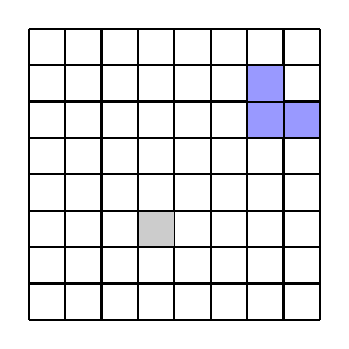
\begin{tikzpicture}[
	thick,
    scale=0.66
]	
	\draw[step=0.7,black] (0.0,0.0) grid (5.6,5.6);
	\node[rectangle,anchor=north west,minimum width=0.44cm,minimum height=0.44cm,fill=gray!40] at (2.1,2.1) {};
	\node[rectangle,anchor=north west,minimum width=0.44cm,minimum height=0.44cm,fill=blue!40] at (4.2,4.2) {};
	\node[rectangle,anchor=north west,minimum width=0.44cm,minimum height=0.44cm,fill=blue!40] at (4.9,4.2) {};
	\node[rectangle,anchor=north west,minimum width=0.44cm,minimum height=0.44cm,fill=blue!40] at (4.2,4.9) {};
\end{tikzpicture}
}
\end{frame}



%-------------------------------------------------------------------------
\begin{frame}{Knight tour}

\vspace{-9pt}
\begin{myboxtitle}[Problema]
 Si consideri ancora una scacchiera $n \times n$; lo scopo è trovare un “giro di
cavallo”, ovvero un percorso di mosse valide del cavallo in modo che ogni
casella venga visitata al più una volta
\end{myboxtitle}

\IG{0.45}{girocavallo.pdf}
\end{frame}

%-------------------------------------------------------------------------
\begin{frame}{Knight tour}

\vspace{-9pt}
\begin{myboxtitle}[Soluzione]
Matrice $n \times n$ le cui celle contengono: 
	\BIL
  \item $0$	\qquad	se la cella non è mai stata visitata
  \item $i$	\qquad	se la cella è stata visitata al passo $i$-esimo
	\EIL
\end{myboxtitle}

\end{frame}

%-------------------------------------------------------------------------
\begin{frame}{Knight tour}

\vspace{-9pt}
\begin{Procedure}
\caption[A]{\BOOLEAN \fontproc{knightTour}($\INTEGER[\,][\,]\ S$, \INTEGER $i$, \INTEGER $x$, \INTEGER $y$)}
\Comment{Se $i=64$, ho fatto 63 mosse e ho completato un tour (aperto)}
\If{$i \Eq 64$}
{
  $\processSolution(S)$\;
  \Return \TRUE\;
}{
  $\Set\ C = \fontproc{moves}(S, x, y)$\;
  \ForEach{$c \in C$}
  {
    $S[x][y] = i$\;
    \If{$\fontproc{knightTour}(S, i+1, x + m_x[c], y + m_y[c])$}{
      \Return \TRUE;
    }
    $S[x][y] = 0$\;
  }
  \Return \FALSE\;
}
\end{Procedure}

\end{frame}

%-------------------------------------------------------------------------
\begin{frame}{Knight tour}

\vspace{-9pt}
\begin{Procedure}
\caption[A]{\Set \fontproc{moves}($\INTEGER[\,][\,]\ S$, \INTEGER $x$, \INTEGER $y$)}
$\Set\ C = \setconstructor()$\;
\For{ $i = 1$ \TO $8$}{
  $n_x = x + m_x[i]$\;
  $n_y = y + m_y[i]$\;
  \If{$1 \leq n_x \leq 8$ \AND $1 \leq n_y \leq 8$ \AND $S[n_x][n_y] \Eq 0$}{
    $C.\setinsert(i)$\;
  }
}
\Return $C$\;
\end{Procedure}

\RestyleAlgo{plain}
\begin{Procedure}
	$m_x = \{ -1, +1, +2, +2, +1, -1, -2, -2 \}$\;
	$m_y = \{ -2, -2, -1, +1, +2, +2, +1, -1 \}$\;
\end{Procedure}

\end{frame}


%-------------------------------------------------------------------------
\begin{frame}{Knight tour -- Considerazioni su efficienza}

\BIL

\item Ad ogni passo ho al massimo $8$ caselle possibili, quindi ne visito al più $8^{63} \approx 7.84 \cdot 10^{55}$
\item Grazie al pruning ne visito molto meno, ma resta comunque un problema
non affrontabile per valori grandi di $n$
\item \EE un esempio del più generale "problema del cammino hamiltoniano", per il quale non esistono soluzioni polinomiali
\item Per questo particolare problema, tuttavia, esistono degli algoritmi di
costo lineare nel numero di caselle, basati su divide-impera
\EIL

\end{frame}

%-------------------------------------------------------------------------
\begin{frame}{Generazione labirinti}

\TwoCols{
\BB{Problemi}
\BIL
\item Come generare un labirinto in una griglia $n \times n$?
\item Come uscire da un labirinto?
\EIL
}{
\vspace{-12pt}
\IG{1.0}{maze.pdf}
}
\end{frame}


\section{Backtracking iterativo}

\subsection{Inviluppo convesso}

%-------------------------------------------------------------------------
\begin{frame}{Inviluppo convesso (Convex Hull)}

\vspace{-12pt}
\TwoCols{
\begin{myboxtitle}[Poligono convesso]
Un poligono nel piano è \alert{convesso} se ogni segmento di retta che
congiunge due punti del poligono sta interamente nel poligono stesso (bordo incluso).
\end{myboxtitle}
}{
\begin{myboxtitle}[Inviluppo convesso]
Dati $n$ punti $p_1, \ldots, p_n$ nel piano, con $n \geq 3$, l'\alert{inviluppo convesso}
(\alert{convex hull}) è, fra tutti i poligoni convessi che li contengono tutti, quello di superficie minima.
\end{myboxtitle}
}

\medskip
\IG{1.0}{16-back-geometry1.pdf}

\end{frame}


%-------------------------------------------------------------------------
\begin{frame}{Algoritmo inefficiente -- $O(n^3)$}

\BIL
\item Un poligono può essere rappresentato per mezzo dei suoi spigoli
\item Si consideri la retta che passa per una coppia di punti $p_i,p_j$, che divide il piano in due semipiani chiusi ($O(n^2)$ coppie)
\item Se tutti i rimanenti $n-2$ punti stanno "dalla stessa parte", allora lo
spigolo $S_{ij}$ fa parte dell’inviluppo convesso
\EIL
\IG{0.8}{16-back-geometry2.pdf}

\end{frame}

%-------------------------------------------------------------------------
\begin{frame}{"Stessa parte"}

\vspace{-15pt}
\TwoColsCustom{0.65}{0.32}{
\begin{myboxtitle}[Problema]
Data una retta definita dai \alert{punti $p_1$ e $p_2$}, determinare se due \alert{punti $p$ e $q$} 
stanno nello \alert{stesso semipiano} definito dalla retta.
\end{myboxtitle}
}{
\vspace{15pt}
\scalebox{0.9}{
\includestandalone{figs/16/sameside}
}
}

\begin{Procedure}
\caption[A]{\BOOLEAN\ \textsf{sameSide}(\Point $p_1$, \Point $p_2$, \Point $p$, \Point $q$)}
\REAL\ $dx = p_2.x - p_1.x$\;
\REAL\ $dy = p_2.y - p_1.y$\;
\REAL\ $dx_1 = p.x - p_1.x$\;
\REAL\ $dy_1 = p.y - p_1.y$\;
\REAL\ $dx_2 = q.x - p_2.x$\;
\REAL\ $dy_2 = q.y - p_2.y$\;
\Return $((dx \cdot dy_1 - dy \cdot dx_1) \cdot (dx \cdot dy_2 - dy \cdot dx_2) \ge 0)$\;
\end{Procedure}


\end{frame}



%-------------------------------------------------------------------------
\begin{frame}{Algoritmo di Jarvis (Gift Packing) -- $O(nh)$}

\vspace{-12pt}
\TwoCols{
\begin{overprint}
\onslide<1|handout:1>
\BB{Punti 0,1}
\BIL
\item Si assegna a $p_0$ il punto più a sinistra, che appartiene all'inviluppo convesso ($O(n)$)
\item Si calcola l'angolo della retta passante per $p_0$ e ogni altro punto
$p_j$ rispetto alla retta verticale ($O(n)$)
\item Si seleziona come punto $p_1$ il punto con angolo minore (costo $O(n)$)
\EIL
\onslide<2|handout:2>
\BB{Punto $i$}
\BIL
\item Si considera la retta $r$ passante per i punti $p_{i-1}, p_{i-2}$
\item Si calcola l'angolo passante per $p_{i-1}$ e ogni altro punto non 
considerato e la retta $r$
\item Si seleziona come punto $p_i$ il punto con angolo minore 
\item Costo per ogni spigolo: $O(n)$
\EIL
\onslide<3|handout:3>
\BB{Terminazione}
\BIL
\item Si termina quando si torna al punto $p_0$
\item L'algoritmo ha costo $O(nh)$, dove $h$ è il
 numero di spigoli
\EIL
\end{overprint}
}{
\IG{1.0}{jarvis.png}
}

\bigskip
\tiny
\url{https://en.wikipedia.org/wiki/Gift_wrapping_algorithm\#/media/File:Jarvis_march_convex_hull_algorithm_diagram.svg}

\end{frame}





%-------------------------------------------------------------------------
\begin{frame}{Algoritmo di Graham}

\vspace{-9pt}
\begin{myboxtitle}[Fase 1]
\BIL
\item Il punto con ordinata minima fa parte dell’inviluppo convesso
\item Si ordinano i punti in base all’angolo formato dalla retta passante per il punto con ordinata minima e la retta orizzontale
\EIL
\end{myboxtitle}

\IG{0.55}{16-back-geometry3.pdf}

\end{frame}

%-------------------------------------------------------------------------
\begin{frame}{Algoritmo di Graham}

\begin{Procedure}
\caption[A]{\Stack \graham($\Point[\,]\ p$, \INTEGER $n$)}
\INTEGER $\Min = 1$\;
\For{$i = 2$ \TO\ $n$}{
  \If{$p[i].y < p[\Min].y$}{$\Min = i$}
}
$p[1] \leftrightarrow p[\Min]$\;
\{ riordina $p[2, \mldots n]$ in base all'angolo formato rispetto all'asse orizzontale quando sono connessi con $p[1]$ \}\;
\{ elimina eventuali punti “allineati” tranne i più lontani da $p_1$, aggiornando $n$ \}\;
[...]\;
\end{Procedure}


\end{frame}

%-------------------------------------------------------------------------
\begin{frame}{Algoritmo di Graham}

\vspace{-9pt}
\begin{myboxtitle}[Fase 2]
\BIL
\item Inserisci $p_1,p_2$ nell'inviluppo corrente
\item Per tutti i punti $p_i = 3, \ldots, n$:
\BIL
\item Siano $p_{j-1}$ e $p_j$ il penultimo e ultimo vertice dell'inviluppo corrente
\item Se $\textsf{sameSide}(p_{j-1}, p_{j}, p_1, p_i) = \FALSE$, ovvero $p_1$ e $p_i$ non si trovano dalla stessa parte rispetto alla retta passante per $p_{j-1}$ e $p_j$, allora elimina $p_j$ dall'inviluppo corrente 
\item Termina tale "scansione" se $p_j$ non deve essere eliminato
\item aggiungi $p_i$ all'inviluppo “corrente”
\EIL
\EIL
\end{myboxtitle}

\end{frame}

%-------------------------------------------------------------------------
\begin{frame}{Algoritmo di Graham}

\vspace{-12pt}
\IG{0.65}{16-back-geometry4.pdf}

\end{frame}

%-------------------------------------------------------------------------
\begin{frame}{Algoritmo di Graham}

\vspace{-9pt}
\begin{Procedure}
\caption[A]{\Stack \graham($\Point[\,]\ p$, \INTEGER $n$) (continua)}
$\Stack\ S = \stackconstructor()$\;
$S.\stackpush(p_1); S.\stackpush(p_2)$\;
\For{$i = 3$ \TO\ $n$}{
  \While{\NOT\ $\textsf{sameSide}(S.\stacktop(), S.\stacktopdue(), p_1, p_i)$}{
    $S.\stackpop()$\;
  }
  $S.\stackpush(p_i)$\;
}
\Return $S$\;  
\end{Procedure}

\end{frame}

%-------------------------------------------------------------------------
\begin{frame}{Algoritmo di Graham -- Complessità}

\vspace{-9pt}
\begin{myboxtitle}[Complessità: $O(n \log n)$]
\BI
\item Il calcolo degli angoli richiede $O(n)$
\item L'ordinamento richiede $O(n \log n)$
\item La rimozione di punti con angolo uguale richiede $O(n)$
\item Ogni punto viene aggiunto/rimosso al massimo una volta
(costo $O(n)$)
\EI
\end{myboxtitle}

\end{frame}

%-------------------------------------------------------------------------
\begin{frame}{Conclusioni}

\begin{tabular}{|P{3cm}|P{5.8cm}|P{1.8cm}|}
\hline
\textbf{Algoritmo} & \textbf{Note} & \textbf{Compl.} \\\hline
Gift packing & $h$ numero di punti nell'inviluppo convesso (1973)& $O(nh)$\\\hline
Graham  & Backtracking iterativo (1972)& $O(n \log n)$\\\hline
Monotone Chain  & Come Graham, ma senza angoli (1979) & $O(n \log n)$ \\\hline
Preparata, Hong  & Divide et impera (1977) & $O(n \log n)$ \\\hline
Chan  & Graham + Jarvis (1996) & $O(n \log h)$ \\\hline
\end{tabular}




\end{frame}

%-------------------------------------------------------------------------
\begin{frame}{Conclusioni}


\BB{
“Convex hull is the favorite paradigm
of \alert{computational geometers}.
Although the description of the problem is
fairly simple, its solution takes into account
all aspects of computational geometry.”
}


O. Devillers (1996)

\end{frame}

\end{document}

%---------------------------------------------------------------------------
\begin{frame}{Quale tecnica applicare?}

\vspace{-9pt}
\begin{myboxtitle}[Sottostruttura ottima]
\EE possibile spezzare ricorsivamente un problema in sottoproblemi più piccoli? Le decisioni prese per un problema rimangono valide quando esso diviene un sottoproblema di un problema più grande?
\end{myboxtitle}


\vspace{-9pt}
\begin{columns}[T]
\column{0.45\textwidth}
\BB{Risposta: S\`I}
\BIL
\item Divide-et-impera
\item Prog. dinamica
\item Memoization
\item Greedy
\item Backtrack
\EIL
\column{0.45\textwidth}
\BB{Risposta: NO}
\BIL
\item Backtrack
\item Oppure, risoluzione ad-hoc
\EIL
\end{columns}

\end{frame}

%---------------------------------------------------------------------------
\begin{frame}{Quale tecnica applicare?}

\vspace{-9pt}
\begin{myboxtitle}[Spazio dei sottoproblemi]
Lo spazio dei sottoproblemi ha dimensione superpolinomiale?
\end{myboxtitle}

\vspace{-9pt}
\begin{columns}[T]

\column{0.45\textwidth}
\BB{Risposta: S\`I}
\BIL
\item Backtrack
\EIL

\column{0.45\textwidth}
\BB{Risposta: NO}
\BIL
\item Divide-et-impera
\item Prog. dinamica
\item Memoization
\item Greedy
\EIL

\end{columns}

\end{frame}


\begin{frame}{Quale tecnica applicare?}

\vspace{-9pt}
\begin{myboxtitle}[Ripetizioni]
Lo stesso sottoproblema può occorrere più volte come sottoproblema di un problema più grande?
\end{myboxtitle}

\vspace{-9pt}
\begin{columns}[T]
\column{0.45\textwidth}
\BB{Risposta: S\`I}
\BIL
\item Prog. dinamica
\item Memoization
\item Greedy
\EIL
\column{0.45\textwidth}
\BB{Risposta: NO}
\BIL
\item Divide-et-impera
\item Greedy
\EIL
\end{columns}

\end{frame}

\begin{frame}{Quale tecnica applicare?}

\vspace{-9pt}
\begin{myboxtitle}[Copertura dei sottoproblemi]
\BIL
\item Per risolvere il problema principale, è necessario risolvere tutti i sottoproblemi?
\EIL
\end{myboxtitle}

\vspace{-9pt}
\begin{columns}[T]
\column{0.45\textwidth}
\BB{Risposta: S\`I}
\BIL
\item Prog. dinamica
\item Memoization
\EIL
\column{0.45\textwidth}
\BB{Risposta: NO}
\BIL
\item Greedy
\item Memoization
\EIL
\end{columns}

\end{frame}


\end{document}



